% THIS IS AN EXAMPLE DOCUMENT FOR VLDB 2010
% based on ACM SIGPROC-SP.TEX VERSION 2.7
% Modified by  Gerald Weber <gerald@cs.auckland.ac.nz>


% This example *does* use the .bib file (from which the .bbl file
% is produced). REMEMBER HOWEVER: After having produced the .bbl file,
% and prior to final submission, you need to 'insert'  your .bbl file into
% your source .tex file so as to provide ONE 'self-contained' source file.


\documentclass[a4paper,12pt]{report}
\renewcommand{\baselinestretch}{1.5}
%\usepackage[linesnumbered,boxed]{algorithm2e}
\usepackage{amsmath}
\usepackage{amsthm}
\usepackage{algorithm}
%\usepackage{algorithmic}
\usepackage{algpseudocode}
\usepackage{graphicx}
\usepackage{verbatim}
\usepackage{latexsym}
\usepackage{subfigure}
\usepackage{subfig}
\usepackage{color}
\usepackage{float}
\usepackage{indentfirst}
\usepackage{wallpaper}
\usepackage{pdfpages}
\usepackage{multirow}
\usepackage{enumerate}
\usepackage{url}
%\usepackage{hyperref}

\newtheorem{theorem}{Theorem}


\CenterWallPaper{.30}{figure/nthu-logo.pdf}

%\setCJKmainfont{標楷體}
%\XeTeXlinebreaklocale "zh"
%\XeTeXlinebreakskip = 0pt plus 1pt

\renewcommand{\algorithmicrequire}{\textbf{Input:}}  % Use Input in the format of Algorithm
\renewcommand{\algorithmicensure}{\textbf{Output:}} % Use Output in the format of Algorithm

%set paper size
\special{papersize=8.5in,11in}
\topmargin=14.7mm    %bottom margin 14.7mm
\oddsidemargin=30mm   %left & right margin 17.45mm

%text sizes (Keep these values unchanged!)
\textwidth=150mm \textheight=250mm
\columnsep=5.0mm
\parindent=3.5mm

%misc parameters
\headsep=0mm  \headheight=0mm \footskip=18mm

%conversion to values for LaTeX
\advance\topmargin-1in\advance\oddsidemargin-1in
\evensidemargin\oddsidemargin

\begin{document}
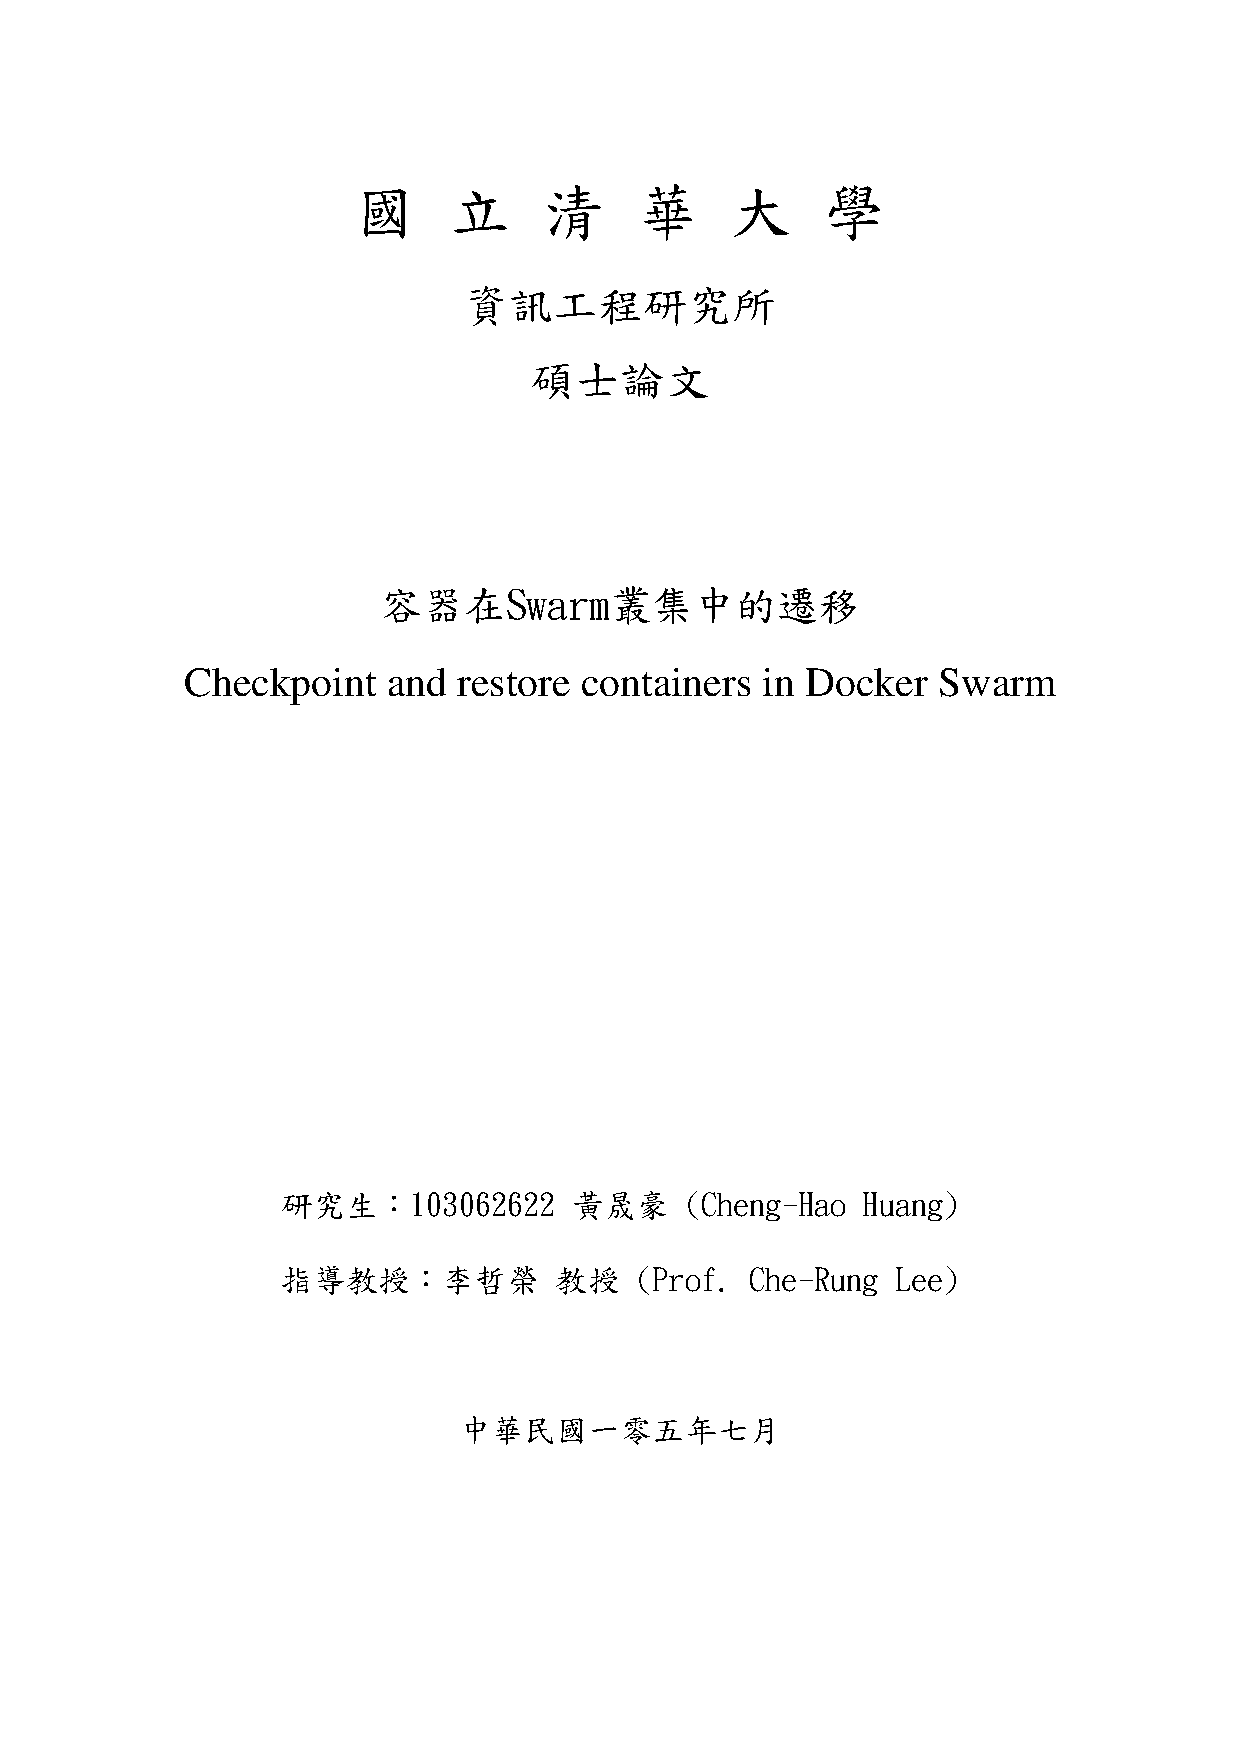
\includepdf[pages={1}]{cover.pdf}
%\includepdf[pages={1}]{cover_ch.pdf}

\title{\bf \huge Container Migration and High Availability in Docker Swarm using Checkpoint and Restoration}

\date{}
\author{
\begin{tabular}{c}
\\
\\
{\LARGE \bf Student: Cheng-Hao Huang}\\
{\LARGE \bf Advisor: Prof. Che-Rung Lee}\\
\\
\\
\\
\\
{\LARGE \bf Department of Computer Science}\\
{\LARGE \bf National Tsing Hua University}\\
{\LARGE \bf Hsinchu, Taiwan, 30013, R.O.C.}\\
\\
{\large July 2016}
\end{tabular}
}

\maketitle
\includepdfset{pagecommand={\thispagestyle{plain}}}
\pagenumbering{roman}
%\addcontentsline{toc}{chapter}{\ctxfr 中文摘要}
\addcontentsline{toc}{chapter}{Chinese Abstract}

\includepdf[pages={1}]{abstract_ch.pdf}

\addcontentsline{toc}{chapter}{Abstract}
\begin{abstract}
\thispagestyle{plain} 
\setcounter{page}{2}

Container becomes a popular technology since Docker has published in 2013.
Container technology has solved programmer and system maintainer when they have to deploy their applications in the servers.
They just need to build the container images, and the container images can run on everywhere they want.
Container technology also isolates each container environments just likes a single host machine.

In this paper, we not only migrate the Docker containers between two physical machines, but also migrate the Docker containers in the Docker Swarm cluster.
Furthermore, we enhance the high availability in the Docker Swarm cluster, the container can be set that checkpoint the container images to remote storage service; whenever the Docker Nodes are fail, the containers which run in the failed Docker Nodes will restore the newest checkpoint to the alive Docker Nodes as well.
\end{abstract}


\setcounter{page}{4}
\addcontentsline{toc}{chapter}{Contents}
\tableofcontents
\clearpage
\addcontentsline{toc}{chapter}{List of Figures}
\listoffigures
\clearpage
\addcontentsline{toc}{chapter}{List of Tables}
\listoftables
\clearpage
\addcontentsline{toc}{chapter}{List of Algorithms}
\listofalgorithms
\clearpage


\pagenumbering{arabic}
\setcounter{page}{1}
\chapter{Introduction}
\label{chap:intro}
Traditionally, people rely single supercomputer to calculate data or deploy their companies' application. Nowadays, cloud computing has been use wildly. People would like to use a lot of normal computers that gather them into a cluster to replace a supercomputer. More and more companies build their data centres or use cloud platforms to construct their business application.
However, the more computers we have, the more power consumption problem we have to solve. At the same time, to make sure every computers' process in the cluster are alive, high availability becomes a more important role in cloud computing.

Virtualization is a popular technology that is used wildly on cloud computing,  including virtual operating system, computer hardware platforms, storage device and computer network resources.
Virtual machine is a technology to emulate a particular computer like a real computer. It can partition a physical machine resource, such as CPU, memory, storage, and network.
A hypervisor uses execution to manage and share host physical machine hardware, it allows many different virtual machines isolated from each other.

Container is operating system level virtualization which runs as an isolated process in userspace on the host operating system and shares the same operation system kernel with other containers.
It provides kernel namespace such as PID, IPC, network, mount, and user namespace to isolate each container environment to host operation system.
In order to control hardware resource like CPU, memory, network, and disk I/O, container uses cgroups to limit each container resources.
Container doesn't have hypervisor to isolate with host operating system, therefore, it can offer better performance than virtual machine. It already has many software to control container, like LXC \cite{helsley2009lxc}, LXD, Open VZ, For now, Docker \cite{Docker} is the most popular container engine. The Virtual Machine and Container architecture is shown as Fig \ref{fig:VM_vs_container}.

\begin{figure}[h]
\begin{center}
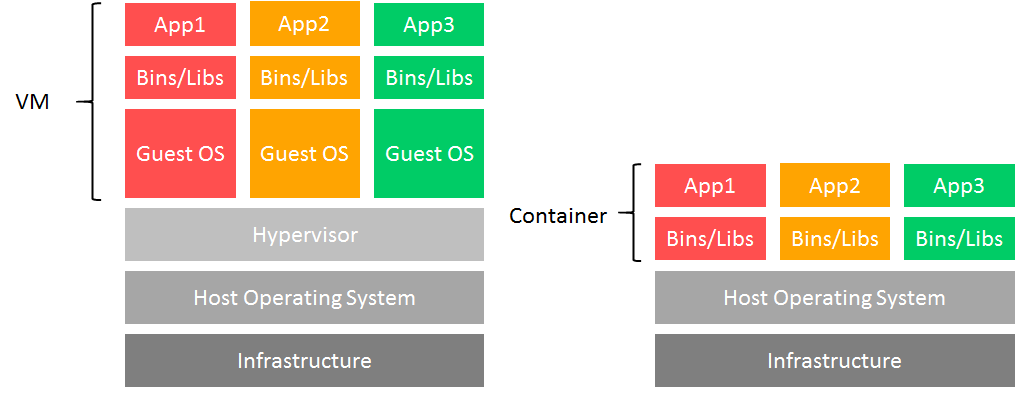
\includegraphics[width=15cm]{figure/VM_vs_container.png}
\end{center}
\caption{Virtual Machine and Container architecture}
\label{fig:VM_vs_container}
\end{figure}

Checkpoint and restoration can freeze a running process state and save process information to checkpoint images. User can use these checkpoint image files to restore the process which user want to restore the process state. These features can be used to dump checkpoint and restore containers because each containers are processes in the host operating system.

In this paper, we choose container but not Virtual Machine to do migration between two host machines, because container need less disk storage and less network transport resources. We not only use checkpoint and restoration to migrate the containers between two physical computers but also migrate the containers in the Docker cluster.
There are many Docker cluster software, like Docker Swarm, Google Kubernetes, Apache Mesos, etc. We choose Docker Swarm because it support native Docker API, and Docker usage habit. We don't need to learn the other Docker cluster software.
Moreover, we improve high availability and rescheduling feature in Docker Swarm using checkpoint and restoration than keep versions of container checkpoint images in remote storage server that whenever computer are fail, Docker Swarm manager will restore the containers from the checkpoint images.

\chapter{Background}
\label{chap:background}
\section{Docker}
Docker is a open-source project container engine. It provides an additional layer of abstraction and automation of operating-system-level virtualization on Linux. Docker engine include Docker client and Docker daemon.
\subsection{Docker client}
Docker is typical Client/Server architecture application. Docker client uses Docker command to send and receive requests to Docker daemon. Also, Docker supports remote RESTful API to send and receive HTTP requests to Docker daemon, it has been implemented by more than 10 programming languages.
\subsection{Docker daemon}
Docker daemon is a daemon that runs as system service. It has two the most importance features: 
\begin{itemize}
    \item Receive and handle Docker client's requests.
    \item Manage containers.
\end{itemize}
When docker daemon is running, it will run a server that receives requests from Docker clients or remote RESTful API. After receives requests, server will pass requests by router to find handler to handle the requests.
\section{Docker Swarm}
Docker Swarm is native clustering for Docker. It gathers several docker engines together into  one virtual docker engine. Docker Swarm serves standard Docker API, so it can be connected by Dokku, Docker Machine, Docker Compose, Jenkins, DockerUI, Drone, etc. And it also support Docker client of course.
In Docker Swarm, It has two components, Include Swarm master and Swarm node. Swarm master is the manager which handles Docker client and RESTful API requests and manages multiple Docker nodes resources. Docker node is an agent which sends heartbeat to discovery server to ensure Docker daemon is alive in the cluster.
\subsection{Discovery services}
Docker Swarm provides multiple discovery services backends. They are used to discovery nodes in the cluster. There are:
\begin{itemize}
    \item Using a distributed key/value store, like Consul, Etcd and Zookeeper.
    \item A static file or list of nodes.
    \item Docker Hub as a hosted discovery service
\end{itemize}
Otherwise, It also supports any modules which satisfy discovery API interface.
\subsection{Scheduler}
Docker Swarm scheduler decides which nodes to use when creating and running a container. It has two steps. First, It follows user's filters to decide which nodes are conform. Second, It passes through strategies to select the best node in the cluster.
\subsubsection{Filter}
Filters are divided into two categories, node filters and container configuration filters. Node filters operate on characteristics of the Docker host or on the configuration of the Docker daemon. Container configuration filters operate on characteristics of containers, or on the availability of images on a host.
The node filters are:
\begin{itemize}
    \item constraint
    \item container slots
    \item health filter
\end{itemize}
The container configuration filters are:
\begin{itemize}
    \item affinity
    \item dependency
    \item port filter
\end{itemize}
\subsubsection{Strategies}
The Docker Swarm scheduler features multiple strategies for ranking nodes. Swarm currently supports these values:
\begin{itemize}
    \item spread
    \item binpack
    \item random
\end{itemize}
Spread and binpack strategies compute rank according to a node’s available CPU, its RAM, and the number of containers it has. It selects a node at random. Under the spread strategy, Swarm optimizes for the node with the least number of containers. The binpack strategy causes Swarm to optimize for the node which is most packed. The random strategy uses no computation, chooses nodes at random regardless of their available CPU or RAM.
\subsection{High availability}
In Docker Swarm, Swarm manager responses the cluster and manages the resources of multiple Docker nodes at scale. If Swarm master dies, we have to create a new one and deal with the interruption of service.
The High availability feature allows Docker swarm has multiple Swarm manager instances. We can create a primary manager and multiple replica instances. If we send requests to replica instances, it will be automatically proxied to the primary manager. In addition, if the primary manager fails, the others replica instances will lead a new primary manager.
\section{CRIU}
CRIU stands for Checkpoint and Restore in User Space, creates a complete snapshot of the state of a process, including things like memory contents, file descriptors, and even open tcp connections. It can be used for suspending and resuming processes, or live migrating them from one machine to another.

\ref{chap:background} and cite test \cite{Knight:1986:AMF:319838.319854, Sohi:1995:MP:225830.224451, Hammond:1998:DSS:291069.291020}.
\chapter{Design and Implementation}
\label{chap:design}
\section{Docker}
In native Docker, It has two part, Docker Client and Docker Daemon. Docker Daemon has many components include server, engine, registry, graph, driver and runC. To  support dump checkpoint and restore request, some of these steps should be implemented.

\subsection{Docker Client}
We implement 3 Docker commands in Docker Client, including checkpoint, restore, migrate. In checkpoint command should have these configurations:
\begin{itemize}
	\item image directory - Dump checkpoint image directory.
	\item work directory - Dump checkpoint image log directory.
	\item leave running - After dumping checkpoint image, keeping running container or not.
	\item pre-dump - Pre-dump checkpoint memory image to minimize frozen time.
	\item pre image directory - Define which version image to compare.
	\item track memory - Track memory to pre image directory image to minimize disk space.
\end{itemize}
In restore command should have these configurations:
\begin{itemize}
	\item image directory - Checkpoint image directory to restore from.
	\item work directory - Directory for restore log.
	\item force - Fore restoring container from image directory whether container is running or not.
\end{itemize}
In migrate command, it focus on Docker Swarm Scheduler filter configurations. In run command, we can do this with the environment variable or the label. Therefore, we implement environment variable and the label configurations in migrate command.

\subsection{Docker Daemon}
In native Docker Daemon, it doesn't support checkpoint and restore command.
Fortunately, it is already implemented in runC, so we have to add some code to proxy Docker Client's requests through Docker Daemon to runC.

\section{Docker Swarm configuration}
As Figure \ref{fig:Docker Swarm with remote storage server}, we prepare a remote storage server for saving Docker containers dump checkpoint images. It should have fault tolerant to avoid service shout down. For these reasons, We choose glusterFS to be our experiments remote storage server.                            

After setting up glusterFS, we mount it to every Docker nodes in the same folder. To avoid mount it as absolute path in every Docker nodes, we mount it to Docker root which we can change configuration in Docker Daemon.

\begin{figure}[h]
\begin{center}
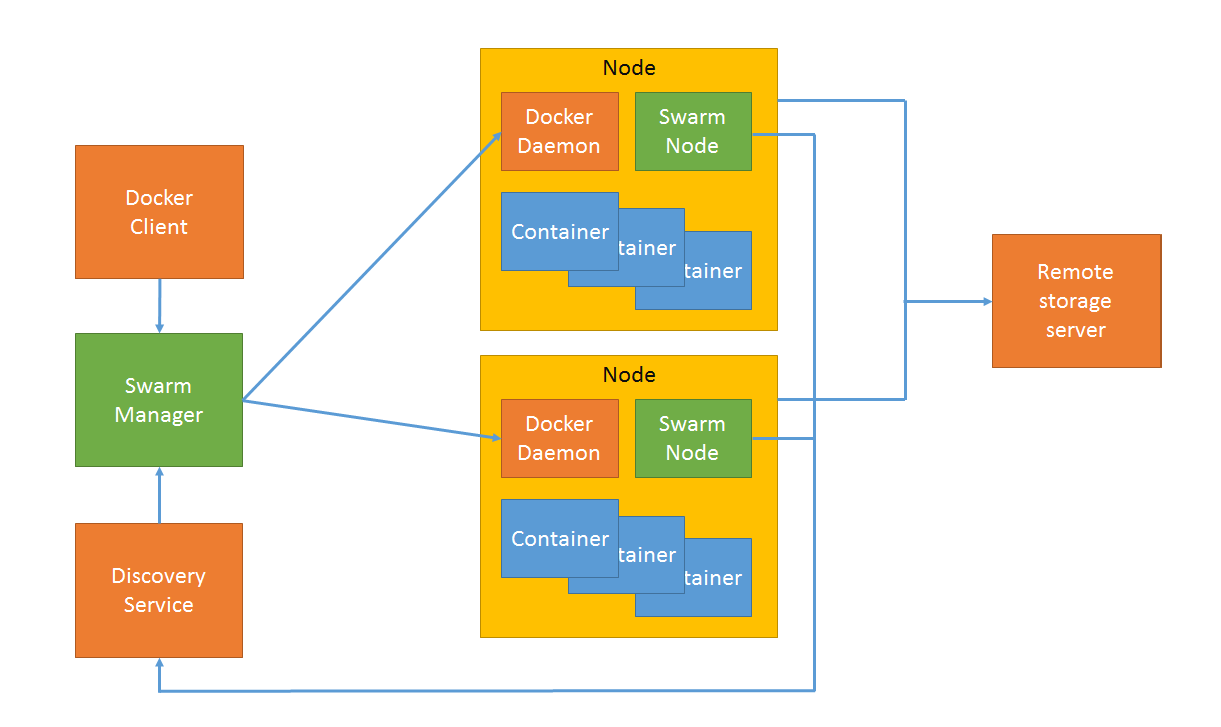
\includegraphics[width=15cm]{figure/swarm_docker_remote.png}
\end{center}
\caption{Docker Swarm with remote storage server}
\label{fig:Docker Swarm with remote storage server}
\end{figure}

\section{Docker containers migration in Docker Swarm}
Docker Swarm creates containers through Swarm scheduler to dispatch Docker nodes. If we want to specific assign which node we want to create containers, we have to set filters like constraint, affinity or dependency.
To migrate containers in Docker Swarm, we must avoid the containers which we want to migrate that migrate to an other nodes, instead of the same node.
\begin{enumerate}[Step 1.]
	\item Check Docker Swarm cluster has at least two Swarm nodes.
    \item Parse Docker Client requests to analyse label and environment variables, and transform label and environment variables to Docker Swarm filters.
    \item Add constraint filter to make sure the container which we want to migrate does not migrate to the same node.
    \item Pre-dump the container checkpoint image which we want to migrate to decrease container frozen time.
    \item Dump the container checkpoint image by tracking memory from pre-dump checkpoint image.
    \item Create empty container on the Docker Swarm scheduler chooses node.
    \item Restore the container to the Docker Swarm scheduler chooses node.
    \item Delete the checkpoint images.
    \item If the container was migrated which had setted checkpoint restore rescheduling policy, it will restart checkpoint restore rescheduling policy \ref{sec:checkpoint restore rescheduling policy}.
\end{enumerate}

\section{Docker Swarm checkpoint restore rescheduling policy}
\label{sec:checkpoint restore rescheduling policy}
In Docker Swarm, it has rescheduling policy. As we set the reschedule policy when we start a container, whenever Swarm nodes fail, Swarm Manager will restart the containers which on the fail nodes to another alive Swarm Nodes.

We improve this policy that we checkpoint every containers which we want to keep checkpoint for every checkpoint ticker. Whenever Swarm Nodes fail, Swarm Manager will restore the containers which Swarm manager has dumped checkpoint. Otherwise, restore rescheduling policy provides version checkpoint by memory track. It only dump different memory page checkpoint to new version checkpoint.

In addition, it also support high availability that whenever Docker Swarm primary manager fails, the others Swarm Manager replica instances will lead a new primary manager. After replica leading a new primary manager, it will restart container checkpoint tickers.
%By experment, it can save at least XX% hard disk space

\subsection{Docker Swarm container checkpoint tickers}
\begin{enumerate}[Step 1.]
	\item Set checkpoint-time label and keep version label when we create the container.
    \item Swarm Manager analyzes checkpoint label when the container has created. If keep version label isn't setted, keep version will be setted to 5.
    \item After the container starting, starting the container checkpoint ticker. Container checkpoint tickers are for when users want to checkpoint container repeatedly at regular intervals. Container checkpoint tickers will do these steps:
    \begin{enumerate}[Step a.]
    \item Swarm Manager sends pre-dump checkpoint request to Swarm Node's Docker Daemon when every Pre-dump version start.
    \item After pre-dumping the container, Swarm Manager sends dump new version checkpoint request to Swarm Node's Docker Daemon. Every new checkpoint images track memory to last checkpoint version image, just save memory difference in new checkpoint image. We save keep-version(default 5) versions in the same directory(Figure \ref{fig:Containers checkpoint versions in remote storage server}).
    \item Send delete checkpoint request to Swarm Node's Docker Daemon to delete last Pre-dump version directory whenever container has two Pre-dump versions.
    \end{enumerate}
\end{enumerate}
\begin{figure}[h]
\begin{center}
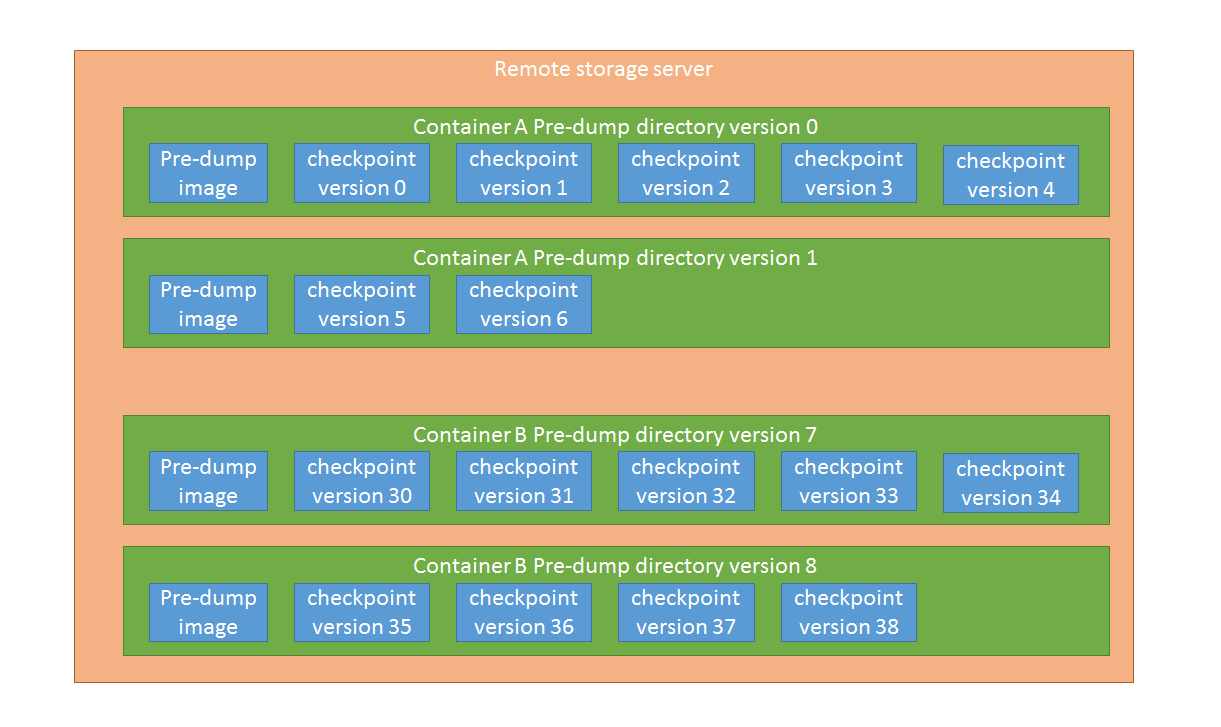
\includegraphics[width=15cm]{figure/checkpoint_demo.png}
\end{center}
\caption{Containers checkpoint version in remote storage server}
\label{fig:Containers checkpoint versions in remote storage server}
\end{figure}
\subsection{Docker Swarm restore rescheduling policy}
\begin{enumerate}[Step 1.]
	\item Set reschedule:restore label when we create the container.
	\item Swarm Manager analyzes restore label when the container start.
    \item Whenever Swarm Nodes fail, Swarm Manager will restore the containers which Swarm Manager has dumped checkpoint last version to another Swarm nodes.
    \item To avoid dumping checkpoint version failing at the same time, if restoring last version failing, Swarm Manager will retry second last version checkpoint to restore. It will retry keep-version(default 5) times.
    \item If Swarm Manager retries keep-version are all fail, it will create and start a new container as normal Docker Swarm rescheduling policy.
\end{enumerate}

\subsection{High availability of Swarm Manager in Docker Swarm checkpoint restore rescheduling policy}
Whenever Docker Swarm primary manager fails, the others Swarm Manager replica instances will lead a new primary manager. After replica leading a new primary manager, it searching every Docker Node's containers which has checkpoint restore rescheduling policy's label. If the containers has checkpoint restore rescheduling policy's label, Docker Swarm new primary manager will restart container checkpoint tickers.
\chapter{Experiments}
\label{chap:experiments}
\section{Environment}
We developed our experiments environment cluster were listed as table \ref{talbe:Host}, and created 4 virtual machines in the computer that each of their resource were listed as table \ref{talbe:Virtual Machine}. We will mount NFS to each virtual machines and test 2 types each of NFS, hard disk, and memory(tmpfs). 
In addition, we will test the difference between \textbf{Direct} method that is defined as new checkpoint image and \textbf{Track-memory} method that is defined as pre-dump checkpoint image which is followed by checkpoint images.

\begin{table}[hbtp]
\begin{center}
\begin{tabular}{|c|c|} \hline
CPU & Intel Xeon(R) CPU-E5-2630 v3 @ 2.40GHz x 32 \\ \hline
Memory & 64 GB \\ \hline
Disk & 1.0 TB \\ \hline
OS & Ubuntu 15.10 64 bit \\ \hline
Kernel version & 4.4.4-040404-generic \\ \hline
Docker version & 1.10.3 \\ \hline
Docker Swarm version & 1.2 \\ \hline
Virtual Box version & 5.10.14 \\ \hline
\end{tabular}
\end{center}
\caption{Experiment environment}
\label{talbe:Host}
\end{table}

\begin{table}[hbtp]
\begin{center}
\begin{tabular}{|c|c|} \hline
CPU & Intel Xeon(R) CPU-E5-2630 v3 @ 2.40GHz x 4 \\ \hline
Memory & 8 GB \\ \hline
Disk & 40 GB \\ \hline
OS & Ubuntu 15.10 64 bit \\ \hline
Kernel version & 4.4.4-040404-generic \\ \hline
Docker version & 1.10.3 \\ \hline
Docker Swarm version & 1.2 \\ \hline
\end{tabular}
\end{center}
\caption{Virtual Machine experiment environment}
\label{talbe:Virtual Machine}
\end{table}

\section{Container Migration Time}
As shown in Figure \ref{fig:Docker Swarm migration time with remote storage server}, native is a based line of the other kinds of experiment.
We choose Redis\cite{paksula2010persisting} as our migration container, because it uses memory to save its data. Therefore, we can check the correctness of Redis data to make sure container migration is success.

In the beginning, creating the container on another Swarm Nodes is fast for all environments because we assume that they have downloaded their container images from the remote repository, thus, they do not need to transport container images from the other Swarm Nodes.

Next, in \textbf{Track-memory} method, the container has to pre-dump the checkpoint image at the version-group created. After pre-dumping the checkpoint image, dumping checkpoint will track memory different with the pre-dump checkpoint image.
On the other hand, \textbf{Track-memory} method, checkpoint ticker dumps the checkpoint image directly.
The result of total checkpoint time, \textbf{Track-memory} method is longer than the other one, because it has to add pre-dumping checkpoint time and dumping checkpoint time.
Although \textbf{Track-memory} method is longer, but it provides the less frozen time to the container that improves CPU's utilization.

Third, Restoring the container to the container which has already been created in the Swarm Node. Except NFS with memory, they all have nearly performance.

Final, it has big disparity of the delete checkpoint image step at \textbf{Track-memory} method, because it has more image files and directories than the version without pre-dumping version.

After all, the checkpoint and restoration of container in memory is faster than hard disk in NFS.
As result of Figure \ref{fig:Docker Swarm migration time with remote storage server}, NFS with memory has the best performance in this experiment.

\begin{figure}[hbtp]
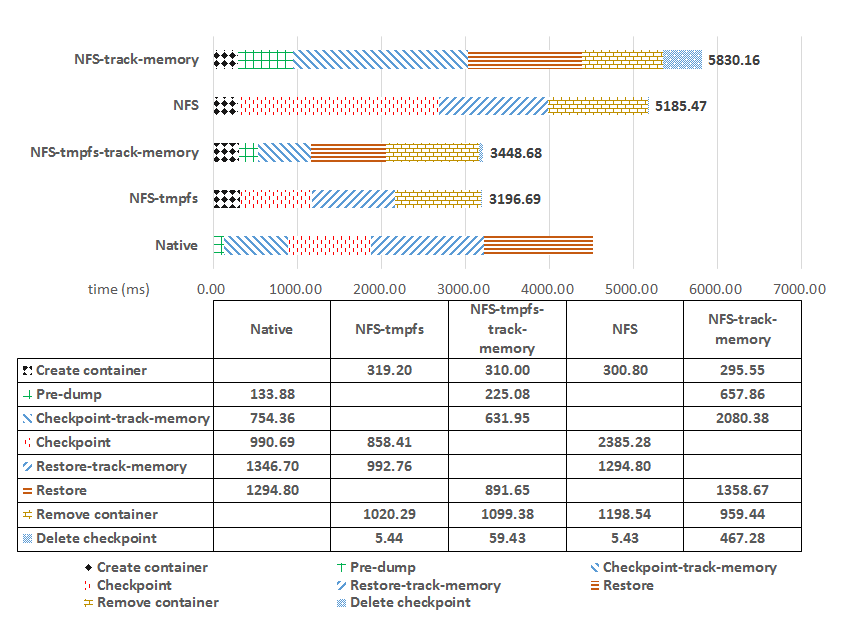
\includegraphics[width=17cm]{figure/migration_time.png}
\caption{Docker Swarm migration with remote storage server}
\label{fig:Docker Swarm migration time with remote storage server}
\end{figure}

\section{The Influence of Container Checkpoint Time on Container Process Time}
\label{sec:CPU Time}
In this experiment, sysbench\cite{kopytov2004sysbench} is used to test performance of process's CPU execution time. Our parameter of sysbench is:
\begin{center}
sysbench --test=cpu --cpu-max-prime=200000 run
\end{center}
It needs to run around 11 minutes in native container without dumping any checkpoint to find the 200000th prime number.

In Figure \ref{fig:Checkpoint Time CPU}, this figure lists every checkpoint time in the experiment environments, also, if remote storage uses the memory to save the checkpoint images, it will get better performance.
In the checkpoint restore rescheduling policy (section \ref{sec:checkpoint restore rescheduling policy}), we set a parameter of checkpoint-ticker period $ T_i $ which will checkpoint repeatedly for every checkpoint-ticker over.

As Figure \ref{fig:Checkpoint Time Influence CPU}, the result of the checkpoint-ticker period $ T_i $ is in direct ratio to the container process execution time.
As these experiment results, the checkpoint-ticker period $ T_i $ has a big influence of container execution time, it is an important parameter in checkpoint restore rescheduling policy that if $ T_i $ is too small, the container will get a bad performance. But if $ T_i $ is too big, whenever Swarm Node fails, the restore container needs to execute the process again. The worst, it might lose some important data. However, no matter the total checkpoint time in \textbf{Track-memory} method, the process's execution time are nearly 
\textbf{Direct} method. This situation shows that the pre-dump checkpoint time has no influence on the process's execution time.

\begin{figure}[hbtp]
\begin{center}
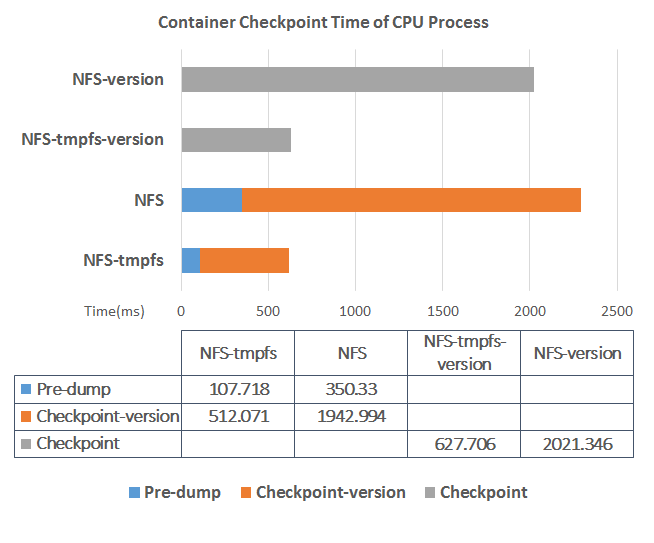
\includegraphics[width=14cm]{figure/cpu_checkpoint_time.png}
\end{center}
\caption{Container checkpoint time of container process time}
\label{fig:Checkpoint Time CPU}
\end{figure}

\begin{figure}[hbtp]
\begin{center}
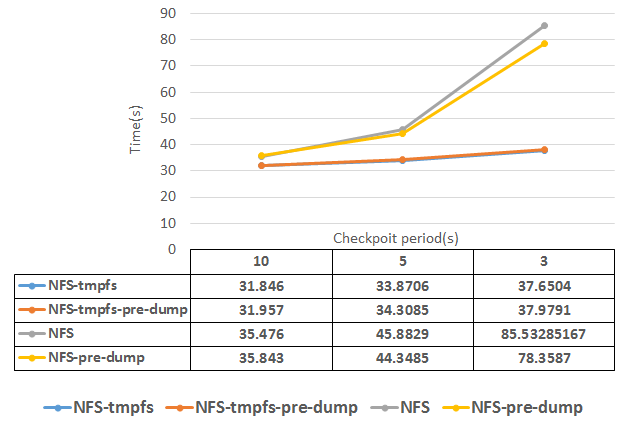
\includegraphics[width=14cm]{figure/cpu_checkpoint_period.png}
\end{center}
\caption{ontainer Checkpoint Time Influence of Container Process Time}
\label{fig:Checkpoint Time Influence CPU}
\end{figure}

\section{The Influence of Container Memory Size on Container Checkpoint Time}
\label{sec:Memory Size}
In this experiment, there are 3 different memory size processes measured. These processes allocate 1 MB, 100 MB, and 1 GB and change the memory with random values quickly in a while loop.

As shown in Figure \ref{fig:1MB}, the pre-dump checkpoint time is at most 1/5 of the checkpoint time and track-memory checkpoint time is about the same as checkpoint time.

However, in Figure \ref{fig:100MB}, the pre-dump checkpoint time is almost a halt of the checkpoint time in the 100 MB process.
In this scenario, the track-memory checkpoint time is still nearly as checkpoint time, but the total checkpoint time is about 1.5 times longer then checkpoint time without track-memory, it means when every version-group is created, the first total checkpoint time is 1.5 times longer then \textbf{Direct} method's checkpoint time .

In the 1 GB process, Figure \ref{fig:1GB} shows that the pre-dump checkpoint time is almost as same as the checkpoint time. It situation shows that the total checkpoint time is about 2 times longer then \textbf{Direct} method when every version-group is created.

In contrast, If the process has allocated the memory but didn't use it, the result will show as Figure \ref{fig:allocate memory}. This figure shows whatever how many memories are allocated in the process, the pre-dump checkpoint time and checkpoint time are all smaller than the process which is allocated memories with changing it.

Follow these experiments, the memory's change has a big influence about container checkpoint time. It is not a effectiveness way when the process need to change memory a lot in the checkpoint-ticker period $ T_i $ time.

\begin{figure}[htbp]
\begin{center}
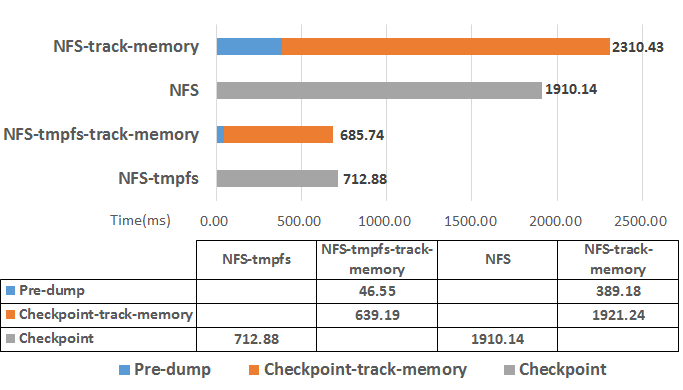
\includegraphics[width=14cm]{figure/1MB.png}
\end{center}
\caption{1MB container process's checkpoint time}
\label{fig:1MB}
\end{figure}

\begin{figure}[htbp]
\begin{center}
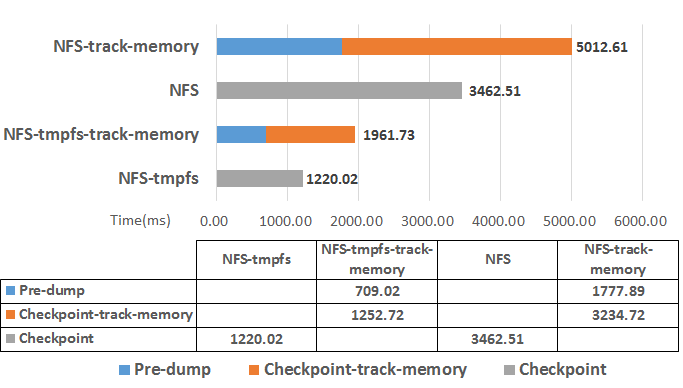
\includegraphics[width=14cm]{figure/100MB.png}
\end{center}
\caption{100MB container process's checkpoint time}
\label{fig:100MB}
\end{figure}

\begin{figure}[htbp]
\begin{center}
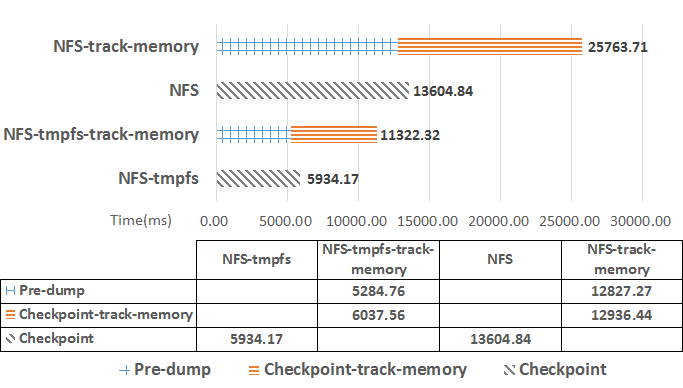
\includegraphics[width=14cm]{figure/1GB.png}
\end{center}
\caption{1GB container process's checkpoint time}
\label{fig:1GB}
\end{figure}

\begin{figure}[htbp]
\begin{center}
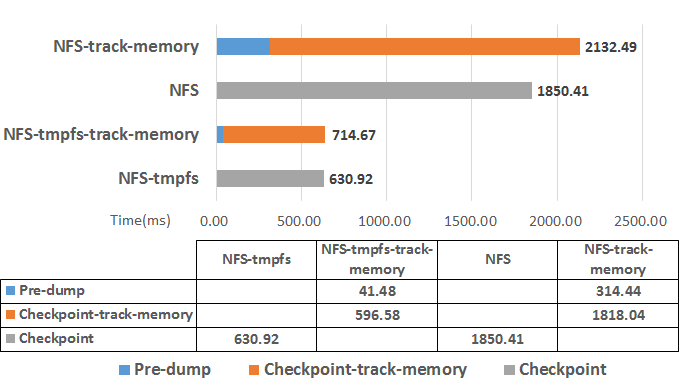
\includegraphics[width=14cm]{figure/allocate_mem_without_change.png}
\end{center}
\caption{Allocated memory without change process's checkpoint time}
\label{fig:allocate memory}
\end{figure}

\section{The Influence of Container Memory Usage on Container Checkpoint Image Size}
In the section \ref{sec:Memory Size}, the container checkpoint time is direct ratio to process memory usage. In this section, the checkpoint images size will be estimated.

In Table \ref{table:process image size}, it shows that the experiments in the section \ref{sec:Memory Size}. If the process uses more memory, the checkpoint image size will be larger. However, although process allocates memory a lot, the checkpoint size still small unless the memory be used.

In Table \ref{table:process image size}, it shows that track-memory version of checkpoint is useless, because it takes more checkpoint time and more storage spaces. To change this view, we test Redis benchmark for daily application. The redis-benchmark command is:
\begin{center}
redis-benchmark -t set -l
\end{center}
This command will send 100000 requests with 50 parallel clients. The results shown as table \ref{table:redis image size}, the pre-dump checkpoint image size is similar as checkpoint image size, but the track-memory checkpoint image size is smaller than the others. This experiment result shows that the Table \ref{table:process image size} is the worst case in checkpoint image size. In this case, if track-memory checkpoint is used, it will save more than 2 times storage space.

As these results, we observe the container checkpoint image size is related with the container checkpoint time.
When the container checkpoint time increasing, the container checkpoint image size will increase, too.
When the container checkpoint image size over 500 MB, it means that the container memory has changed a lot, pre-dump checkpoint is an inefficient action.
To avoid unnecessary container pre-dump, whenever container checkpoint group's average image size over 500 MB, next checkpoint group will not pre-dump the container checkpoint.

\begin{table}[hbtp]
\begin{center}
\begin{tabular}{|c|c|c|c|c|}\hline 
• & 1 MB & 100 MB & 1 GB & Allocate memory without changing\\ 
\hline 
Pre-dump & 1 MB & 100 MB & 1 GB & 102 KB\\ 
\hline 
Checkpoint-track-memory & 1 MB & 100 MB & 1 GB & 90.9 KB \\ 
\hline 
Checkpoint & 1 MB & 100 MB & 1 GB & 175.2 KB \\ 
\hline 
\end{tabular}
\caption{Process allocated memory's checkpoint image size}
\label{table:process image size}
\end{center}
\end{table}

\begin{table}[hbtp]
\begin{center}
\begin{tabular}{|c|c|c|}
\hline 
• & Redis & Redis-benchmark \\ 
\hline 
Pre-dump & 9 MB & 14 MB \\ 
\hline 
Checkpoint-track-memory & 2.3 MB & 2.3 MB \\ 
\hline 
Checkpoint & 9.6 MB & 14 MB \\ 
\hline 
\end{tabular}
\caption{Redis and Redis benchmark's checkpoint image size}
\label{table:redis image size}
\end{center}
\end{table}

\section{The Influence of Many Containers Checkpoint in The Same Time on Container Checkpoint Time}
Figure \ref{fig:many containers} demonstrates the influence of checkpoint time when many containers checkpoint in the same.
As more containers checkpoint in the same time, the more checkpoint time for each container has to take.
In storing in disk case, it almost needs twice times when 4 containers checkpointing in the same time. That's the reason that we implement checkpoint queue to solve this problem.

\begin{figure}[htbp]
\begin{center}
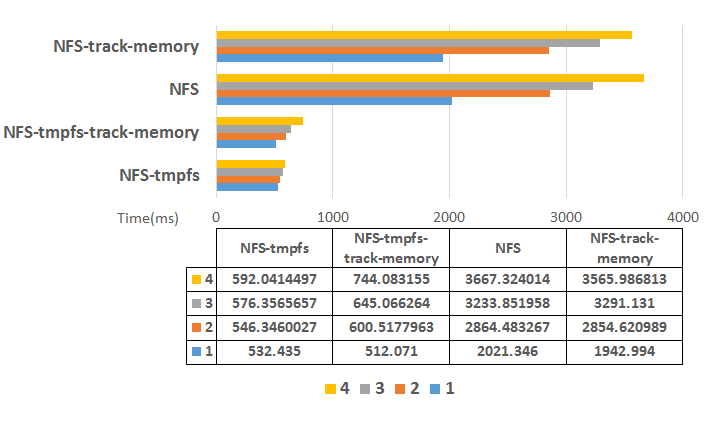
\includegraphics[width=14cm]{figure/many_containers.png}
\end{center}
\caption{Many containers checkpoint in the same time}
\label{fig:many containers}
\end{figure}

\section{The Influence of Container Checkpoint Versions on Container Checkpoint Time}
As Figure \ref{fig:versions}, \textbf{Direct} method's checkpoint time average have 2 horizontal lines.
Two \textbf{Track-memory} method's trendline are slow increasing when the container checkpoint versions growing up.
Each of them has one point of intersections with \textbf{Direct} method's checkpoint time line, the values are and 5 and 16.
Follow these results, checkpoint-version default value sets to 5 is a better choice, and it should not exceed than 16.

\begin{figure}[htbp]
\begin{center}
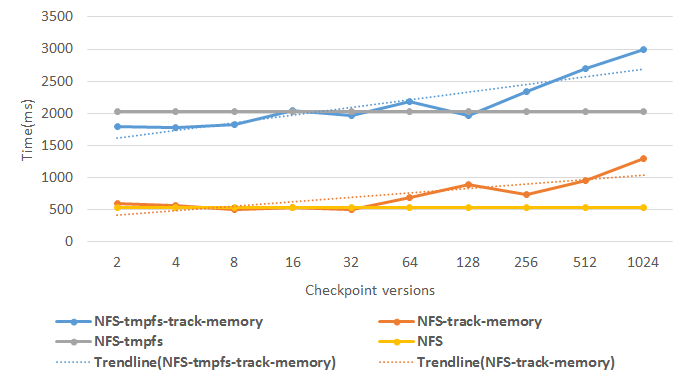
\includegraphics[width=14cm]{figure/versions.png}
\end{center}
\caption{Checkpoint versions of container checkpoint time}
\label{fig:versions}
\end{figure}

\chapter{Related Work}
\label{chap:related}

\cite{hines2009post}
\chapter{Conclusion}
\label{chap:conclusion}
CRIU provides the container for dumping checkpoint and restoring in the same Docker Daemon. In this thesis, we have purposed it to expand to Docker Swarm in the cluster.


\bibliographystyle{plain}
\bibliography{note}

% The following two commands are all you need in the
% initial runs of your .tex file to
% produce the bibliography for the citations in your paper.
%{%\scriptsize
%\bibliographystyle{abbrv}
%\bibliography{HPCoC_cite}
%}
% You must have a proper ".bib" file
%  and remember to run:
% latex bibtex latex latex
% to resolve all references

\end{document}
